\documentclass[a4paper, 10pt]{article}
% (1) Encoding, Fonts, and Layout
\usepackage[T1]{fontenc}
\usepackage{lmodern}
\usepackage[margin=1in]{geometry}


% (2) Common Packages
\usepackage{amsmath, amssymb, amsthm}
\usepackage{xcolor}
\usepackage{caption}
\usepackage{tikz}
\usepackage{pgfplots}
\pgfplotsset{compat=newest}
\usepackage{etoolbox}
\usepackage{tikz-3dplot}
\tdplotsetmaincoords{75}{120}
\usepackage[inline]{enumitem}
\usepackage{bookmark}
\usepackage{mathtools}
\usepackage{subcaption} 
\usepackage[normalem]{ulem}
\usepackage{booktabs,tabularx}
\usepackage{cleveref}
\usepackage[T1]{fontenc}
\usepackage{xcolor}
\usepackage{fontawesome5}
\usepackage{babel}

\usepackage{minted}
\usepackage[most]{tcolorbox}
\tcbuselibrary{theorems}
\tcbuselibrary{listingsutf8, skins}
\usepackage{microtype}

% Patching pgfplots warning
\makeatletter
\patchcmd{\pgfplots@applistXXpushback@smallbuf}{\pgfplots@error}{\pgfplots@warning}{}{}
\makeatother


\definecolor{custom_green}{HTML}{a3be8c}
\definecolor{custom_red}{HTML}{dc322f}
\definecolor{custom_blue}{HTML}{268bd2}
\definecolor{custom_purple}{HTML}{b48ead}

\definecolor{base}{HTML}{eceff4}
\definecolor{gray1}{HTML}{f8f9fa}
\definecolor{gray2}{HTML}{e9ecef}
\definecolor{gray3}{HTML}{2e3440}
\definecolor{off-white}{HTML}{f4f4f6}


% (5) Custom tcolorbox Environments
\newtcbtheorem[number within=section]{definitionbox}{Definition}{%
    enhanced,
    sharp corners,
    attach boxed title to top left={yshift=-0.1mm},
    colback=custom_red!10,
    colframe=custom_red,
    fonttitle=\bfseries,
    boxed title style={
            sharp corners,
            size=small,
            colback=custom_red,
            colframe=custom_red,
        },
    % Put (#1) after the definition number if a name is given
    description delimiters none,
    % Add a line to the ToC whenever the environment begins
    before upper={%
            \addcontentsline{toc}{subsection}{%
                Definition \thetcbcounter\ifstrempty{#1}{}{#1}%
            }%
        }%
}{def}





\newtcolorbox{conceptbox}[1][]{
    title={#1},
    fonttitle=\bfseries\color{white},
    attach boxed title to top left={yshift=-2mm},
    colbacktitle=custom_blue,
    coltitle=white,
    colframe=custom_blue,
    colback=custom_blue!10,
    boxrule=1mm,
    arc=0mm,
    bottomtitle=0.5mm,
    left=2.5mm,
    leftrule=1mm,
    right=3.5mm,
    rightrule=1mm,
    toptitle=1mm,
    enhanced
}

\lstdefinestyle{cStyle}{
    language=C,
    columns=fullflexible,
    tabsize=4,
    keepspaces=true,
    showstringspaces=false,
    numbersep=5pt,
    numbers=left,
    stepnumber=1,
    basicstyle=\ttfamily\small,
    keywordstyle=\bfseries\color{keywordsblue},
    commentstyle=\itshape\color{commentgreen},
    stringstyle=\color{stringspurple},
    frame=none,
    breaklines=true,
    xleftmargin=0.5em,
}

\newtcblisting{codeexample}[2][]{
    listing only,                        
    title=\emph{Example Code:}\quad  \textbf{#2},         
    fonttitle=\bfseries\scriptsize\color{white},
    attach boxed title to top center={yshift=-1.5mm},
    colbacktitle=custom_green,
    coltitle=white,
    colframe=custom_red,
    colback=custom_red!10,
    boxrule=0.5mm,
    arc=0mm,
    bottomtitle=0.5mm,
    left=2.5mm,
    leftrule=0.5mm,
    right=3.5mm,
    rightrule=0.5mm,
    toptitle=1mm,
    enhanced,
    listing options={style=cStyle} 
}



\newtcolorbox{proofbox}[1][]{
    title=\textbf{Proof:} {#1},
    fonttitle=\bfseries\boldmath,
    arc=0mm,
    bottomtitle=0.5mm,
    boxrule=0mm,
    colbacktitle=gray2,
    colback=gray1,
    coltitle=gray3,
    left=2.5mm,
    leftrule=1mm,
    rightrule=1mm,
    right=3.5mm,
    toptitle=0.75mm,
    colframe=custom_blue,
    coltext=gray3,
}

\newtcolorbox{theorembox}[1][]{
    title=\textbf{Theorem} {#1},
    fonttitle=\bfseries\boldmath,
    arc=0mm,
    bottomtitle=0.5mm,
    boxrule=0mm,
    colbacktitle=gray2,
    colback=gray1,
    coltitle=gray3,
    left=2.5mm,
    leftrule=1mm,
    rightrule=1mm,
    right=3.5mm,
    toptitle=0.75mm,
    colframe=custom_green,
    coltext=gray3
}

\newtcolorbox{notebox}{
    title=\textbf{Note},
    fonttitle=\bfseries\boldmath,
    arc=0mm,
    bottomtitle=0.5mm,
    boxrule=0mm,
    colbacktitle=gray2,
    coltitle=gray3,
    left=2.5mm,
    leftrule=1mm,
    rightrule=1mm,
    right=3.5mm,
    toptitle=0.75mm,
    colframe=custom_blue,
    coltext=gray3
}

% \newtcolorbox{examplebox}[1][]{
%     title=\textbf{Example} {#1},
%     fonttitle=\bfseries\boldmath,
%     arc=0mm,
%     bottomtitle=0.5mm,
%     boxrule=0mm,
%     colbacktitle=gray2,
%     colback=gray1,
%     coltitle=gray3,
%     left=2.5mm,
%     leftrule=1mm,
%     rightrule=1mm,
%     right=3.5mm,
%     toptitle=0.75mm,
%     colframe=gray3,
%     fontupper=\footnotesize,
%     coltext=gray3
% }

\newtcbtheorem[number within=section]{examplebox}{Example}{
    enhanced,
    sharp corners,
    attach boxed title to top left={yshift=-0.1mm},
    colback=gray3!10,
    colframe=gray3,
    colbacktitle=gray2,
    fonttitle=\bfseries,
    boxed title style={
            sharp corners,
            size=small,
            colback=gray3,
            colframe=gray3,
        },
    % Put (#1) after the definition number if a name is given
    description delimiters none,
    % Add a line to the ToC whenever the environment begins
    before upper={%
            \addcontentsline{toc}{subsection}{%
                Example \thetcbcounter\ifstrempty{#1}{}{#1}%
            }%
        }%
}{ex}


\theoremstyle{definition}
\newtheorem{definition}{Definition}[section]
\newtheorem{example}[definition]{Example}

\theoremstyle{plain}
\newtheorem{theorem}[definition]{Theorem}

% (7) Hyperlinks
\usepackage{hyperref}
\hypersetup{
    colorlinks=true,    
    linkcolor=black,      
    pdfborder={0 0 0}   
}



% macros.tex
\newcommand{\intinf}{\int_0^{\infty}} % Integral from 0 to infinity
\newcommand{\diff}[2]{\frac{d#1}{d#2}} % Derivative


\usepackage[svgnames]{xcolor}
\usepackage{listings}

\lstset{language=R,
    basicstyle=\footnotesize\ttfamily,
    stringstyle=\color{DarkGreen},
    otherkeywords={0,1,2,3,4,5,6,7,8,9},
    morekeywords={TRUE,FALSE},
    deletekeywords={data,frame,length,as,character},
    keywordstyle=\color{blue},
    commentstyle=\color{DarkGreen},
}

\title{
Robert Davidson \\
\textbf{ST1112: Statistics}
}
\author{
70\% Exam\\
30\% Continuous Assessment (3 parts)
}
\date{}       % Optional: Add date if desired
%--------------------------------------------------------
% Document
%--------------------------------------------------------
\begin{document}
\maketitle
\pagebreak



\tableofcontents
\pagebreak
\section{Descriptive Statisitcs}
\subsection{Sampling the mean}
In \textbf{probability} we consider the underlying process which has some randomness or uncertainity, and we try to figure out what happens \\[2ex]
In \textbf{statistics} we consider the data that we have, and we try to figure out what the underlying process is. The basic aim to infer the population from the sample.
\begin{examplebox}[Consider a jar of red and green jelly beans]
    A probabilist starts by knowing the proportion of red and green jelly beans in the jar, and then tries to figure out the probability of drawing a red jelly bean.\\
    A statistician starts by drawing a sample of jelly beans from the jar, and then tries to figure out the proportion of red and green jelly beans in the jar.
\end{examplebox}

\begin{definitionbox}[ : Central Limit Theorem]
    Sample means follow a normal distrubution, centered on the popular mean, with a standard deviation equal to population standard deviation divided by the square root of the sample size.
    $$\bar{X} \sim N \left(\mu, \frac{\sigma}{\sqrt{n}}\right)$$
\end{definitionbox}

\begin{definitionbox}[ : Standard Error]
    The standard error is the variability in the sampling distrubution. \\
    The standard error describes the typical difference between the sample measurement and the population parameter.
    $$SE = \frac{\sigma}{\sqrt{n}}$$
\end{definitionbox}
\begin{definitionbox}[ : Estimate $\sigma$]
    Often the value of the population standard deviation is unknown, and hence the standard error of the mean is unknown. \\
    We can estimate the value of the standard error using the sample standard deviation $(s)$ as an unbiased estimator of the population standard deviation $(\sigma)$.
    $$\sigma_{\bar{X}} = \frac{s}{\sqrt{n}}$$
\end{definitionbox}


\section{Interential Statistics - Interval Estimation}
\subsection{Confidence Intervals}
\subsubsection{Confidence Intervals for a mean}

\begin{definitionbox}[Confidence Interval for $n > 30$]
    For a large sample size, $n > 30$, a Confidence Interval for the population mean is given by:
    $$\bar{X} \pm Z_{\frac{\alpha}{2}} \frac{s}{\sqrt{n}}$$
\end{definitionbox}
\noindent  A $95\%$ Confidence Interval, $\alpha = 0.05$, meaning we accept a 5\% risk that our interval doesn't contain the true population mean. \\
This $5\%$ is split into $2.5\%$ in each tail of the distrubution : $Z_{\frac{\alpha}{2}} = Z_{0.025}$. \\
When using a normal table that shows "area to the left", we need to find the $Z$ value that corresponds to $1 - 0.025 = 0.975$.
Thus: $Z_{0.025} = 1.96$. \\
$95 \%$ Confidence is most commonly used because increasing the confidence level increases the width of the interval, this may not be useful.


\subsubsection{Confidence Intervals for a small sample size}
When $\sigma$ is known, a 95\% Confidence Interval for the population mean is given by:
$$\bar{X} \pm 1.96  \cdot \frac{\sigma}{\sqrt{n}}$$
When $\sigma$ is unknown, a 95\% Confidence Interval for the population mean is given by:
$$\bar{X} \pm 1.96  \cdot \frac{s}{\sqrt{n}}$$
But, what if $\sigma$ is unknown and $n < 30$?
\begin{definitionbox}[Confidence Interval for $n < 30$]
    For a small sample size, $n < 30$, we use the \textbf{t-distribution instead of the normal distribution}. \\
    The t-distribution has heavier tails than the normal distribution and accounts for the additional uncertainty when estimating $\sigma$ with $s$ in small samples.

    The confidence interval is given by:
    $$\bar{X} \pm t_{\frac{\alpha}{2}} \frac{s}{\sqrt{n}}$$

    Where $t_{\frac{\alpha}{2}}$ is the critical value from the t-distribution with $n-1$ \textbf{degrees of freedom}. \\
    The degrees of freedom represent the \emph{number of independent pieces of information used to estimate the standard deviation}.
    As the degrees of freedom increase, the t-distribution approaches the normal distribution - infinite degrees of freedom is the normal distribution.

    \begin{center}
        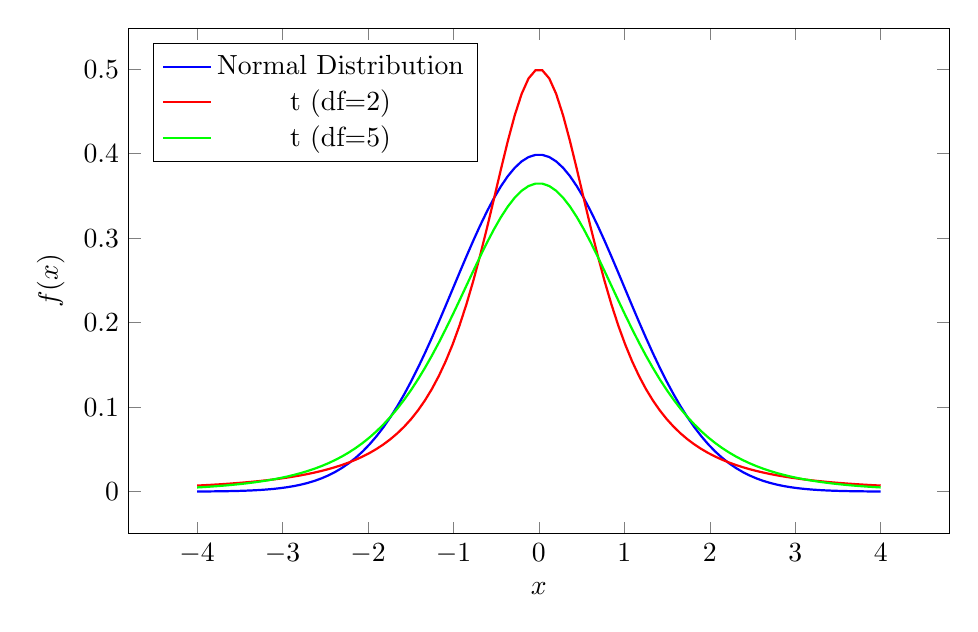
\begin{tikzpicture}
            \begin{axis}[
                    width=12cm,
                    height=8cm,
                    xlabel=$x$,
                    ylabel=$f(x)$,
                    legend pos=north west,
                    samples=100,
                    domain=-4:4
                ]
                % Standard Normal Distribution
                \addplot[blue, thick] {exp(-x^2/2)/sqrt(2*pi)};
                % t-distribution with df=2 (approximated)
                \addplot[red, thick] {0.5/(1+x^2)^1.5};
                % t-distribution with df=5 (approximated)
                \addplot[green, thick] {0.365/(1+x^2/5)^3};

                \legend{Normal Distribution, t (df=2), t (df=5)}
            \end{axis}
        \end{tikzpicture}
    \end{center}
\end{definitionbox}

\begin{examplebox}[: Find t-value from tables For a 95\% Confidence Interval]
    We have:
    $$a = 1 - 0.95 = 0.05 \Rightarrow \frac{a}{2} = 0.025$$
    We also have:
    $$n = 13 \Rightarrow df = 13 - 1$$
    We want to find the $t_{12, 0.025}$ value from the t-distribution table, which is $2.179$.
\end{examplebox}


\subsection{Bootstrap, proportions and counts}
What do we do when our data is not normally distributed? We have two options:
\begin{itemize}
    \item Transform the data to make it normally distributed (e.g. log transformation, square root transformation)
    \item Use a non-parametric method (Bootstrap or CI for the population median)
\end{itemize}


\subsubsection{Bootstrap}
We can quantify the uncertainity in our estimate of the population mean by using the Central Limit Theorem or simulatiuon via the Bootstrap method, as follows:
\begin{enumerate}
    \item Take a bootstrap  sample - random sample taken with replacment from the original sample (same size as original sample)
    \item Calculate the bootstrap statistic - such as mean, median, proportion, etc.
    \item Repeat steps 1 and 2 many times
    \item Calculate the bounds of the 95\% Confidence interval as the middle 95\% of the bootstrap distrubution
\end{enumerate}


\section{Inferential Statistics - Hypothesis Testing}
\subsection{Hypothesis Testing}
A hypothesis test is intended to assess whether a population parameter of interest is equal to some
specified value of direct interest to the researcher \\
Hypothesis tests are structured in a very specific and, what may seem initially, peculiar manner. \\
The p-value is central to the notion of a hypothesis test. \\
The Central Limit Theorem (CLT) and t-distribution provide the framework for assessing how different \\
the sample statistic is from the proposed parameter value.

\subsubsection{Stages in Hypothesis Testing}
\begin{enumerate}
    \item State the null ($H_0$) and alternative ($H_1$) hypotheses
    \item Take a random sample from the populat of interest and calculate a suitable test statistic $(T_0)$ under the assumed model $(H_0)$
    \item Write down the distrubution that the test statistic follows
    \item Investigate how likely the value of the test statistic is if the null hypothesis is true
    \item Make a decision to reject or fail to reject the null hypothesis (using 3 and 4)
    \item Write down the conclusion
\end{enumerate}
The $\textbf{Null Hypothesis}$ is the hypotheses that the population statistic is equal to some claimed value.  \\
The $\textbf{Alternative Hypothesis}$ is the hypotheses that the population statistic is not equal to the claimed value. It must be true if the null hypothesis is false. \\
We asses through a test statistic, how probable (p-value), it would be to observe data as or more extreme than the data we have, if the null hypothesis is true. \\


\end{document}
